\nsection{Sudoku}

This concerns the automated solving of one of the world's most famous puzzles, Sudoku:
\wwwurl{https://en.wikipedia.org/wiki/Sudoku}
\begin{center}
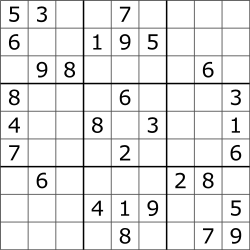
\includegraphics[width=2.5in]{../Pictures/wiki_sudoku.png}
\end{center}

There are many ways to solve such puzzles, some of which are described in:
\wwwurl{https://norvig.com/sudoku.html}


\begin{exercise}
\label{ex:sudoku1}

Using the simple ADT framework provided and the constraint propagation
approach described above, write a program that can solve ``easy'' puzzles.
The constraint propagation approach cannot completely solve ``hard''
puzzles.  A basic ADT is provided for you
in \verb^sudoku.h^, along with a simple test file
\verb^testsudoku.c^.
Write \verb^Fixed/fixed.c^
and \verb^Fixed/specific.h^, so that:

{\small
\begin{terminaloutput}
% make run
Basic Sudoku Tests ... Start
Basic Sudoku Tests ... Stop
Basic Sudoku Tests ... Start
Basic Sudoku Tests ... Stop
\end{terminaloutput}
}
\noindent works correctly. 

\noindent The code will hardwire the grid to be a fixed size $2D$~array,
and be capable of reading in the different files present in \verb^Data/Sudoku^.
Submit a single \verb^.zip^ file which contains your entire submission,
including \verb^Fixed/fixed.c^ and \verb^Fixed/specific.h^.
\end{exercise}

\begin{exercise}
\label{ex:sudoku2}

Extend your program so that all grids are solvable, even the ``hard''
examples given. One typical way to do this is to make a guess for a
square, and then backtrack to undo this if it leads to an incorrect
solution when using constraint propagation.
Efficiency of your solution is not a concern here - focus on creating
beautifully crafted (and tested) code.

\noindent Submit a single \verb^.zip^ file which contains your entire
submission, including the updated versions of \verb^Fixed/fixed.c^
and \verb^Fixed/specific.h^ in addition to \verb^solution.txt^ which
briefly describes the algorithm used.

\end{exercise}

\begin{exercise}
\label{ex:sudoku3}

Extend your program in a manner of your own choosing - this could be a
faster approach to solving all grids (but maybe at the expense of code
readability), exploring Sudokus larger than $9x9$, or allowing better
I/O or user-interaction.

\noindent Submit a single \verb^.zip^ file which contains your entire
submission, including the updated versions of \verb^Fixed/fixed.c^ and
\verb^Fixed/specific.h^ in addition to \verb^extend.txt^ which briefly
describes what you have done.

\end{exercise}

